% !TEX root = main.tex
\section{Measurements and Verification}
\label{sec:verification}
In this section we present measurements and verifications of the proposed system. We first present a verification of the system specifications, such as bandwidth and power, in section \ref{sec:specs_verification}. In section \ref{sec:perf_meas} the system performance will be evaluated under different conditions, and key parameters such as BER and SNR will be presented. In all measurements, the transmit power is kept at $\paPower \si{dBm}$.

\subsection{Verification of System Parameters}
\label{sec:specs_verification}
The verified system specifications is summarised in table \ref{tab:meas_specs}.
% !TEX root = main.tex
\begin{table}[htbp]
  \centering
  \caption{Summarised Measurements of System Parameters}
    \begin{tabular}{lc}
    \rowcolor[rgb]{ 0,  0,  0} \textcolor[rgb]{ 1,  1,  1}{\textbf{System Parameter}}	& \textcolor[rgb]{ 1,  1,  1}{\textbf{Measured Value}} 		\\
    	Half-Power Bandwidth										& \SI{\measBW}{kHz}					\\
    	PA power, $P_{PA}$ 											& \SI{\measPWR}{dBm}					\\
    	Delay 													& \SI{\measDelay}{ms} 					\\
 \end{tabular}
  \label{tab:meas_specs}
\end{table}

The signal bandwidth was analyzed using MATLAB's signal analyzer toolbox \cite{signalAnalyzer}. The resulting power spectrum is shown in figure \ref{fig:pwr_spectrum}. The half-power bandwidth is measured to $\measBW \si{kHz}$.
The transmit power was verified by first calibrating the USRP power spectral density using a spectrum analyser, and then calculating the total transmit power from measured bandwidth\footnote{Due to the CIVID-19 situation the lab equipment was not available for measurements on the implemented system}. This way, the transmit power was measured $\measPWR \si{dBm}$.

\begin{figure}[htbp]
\begin{center}
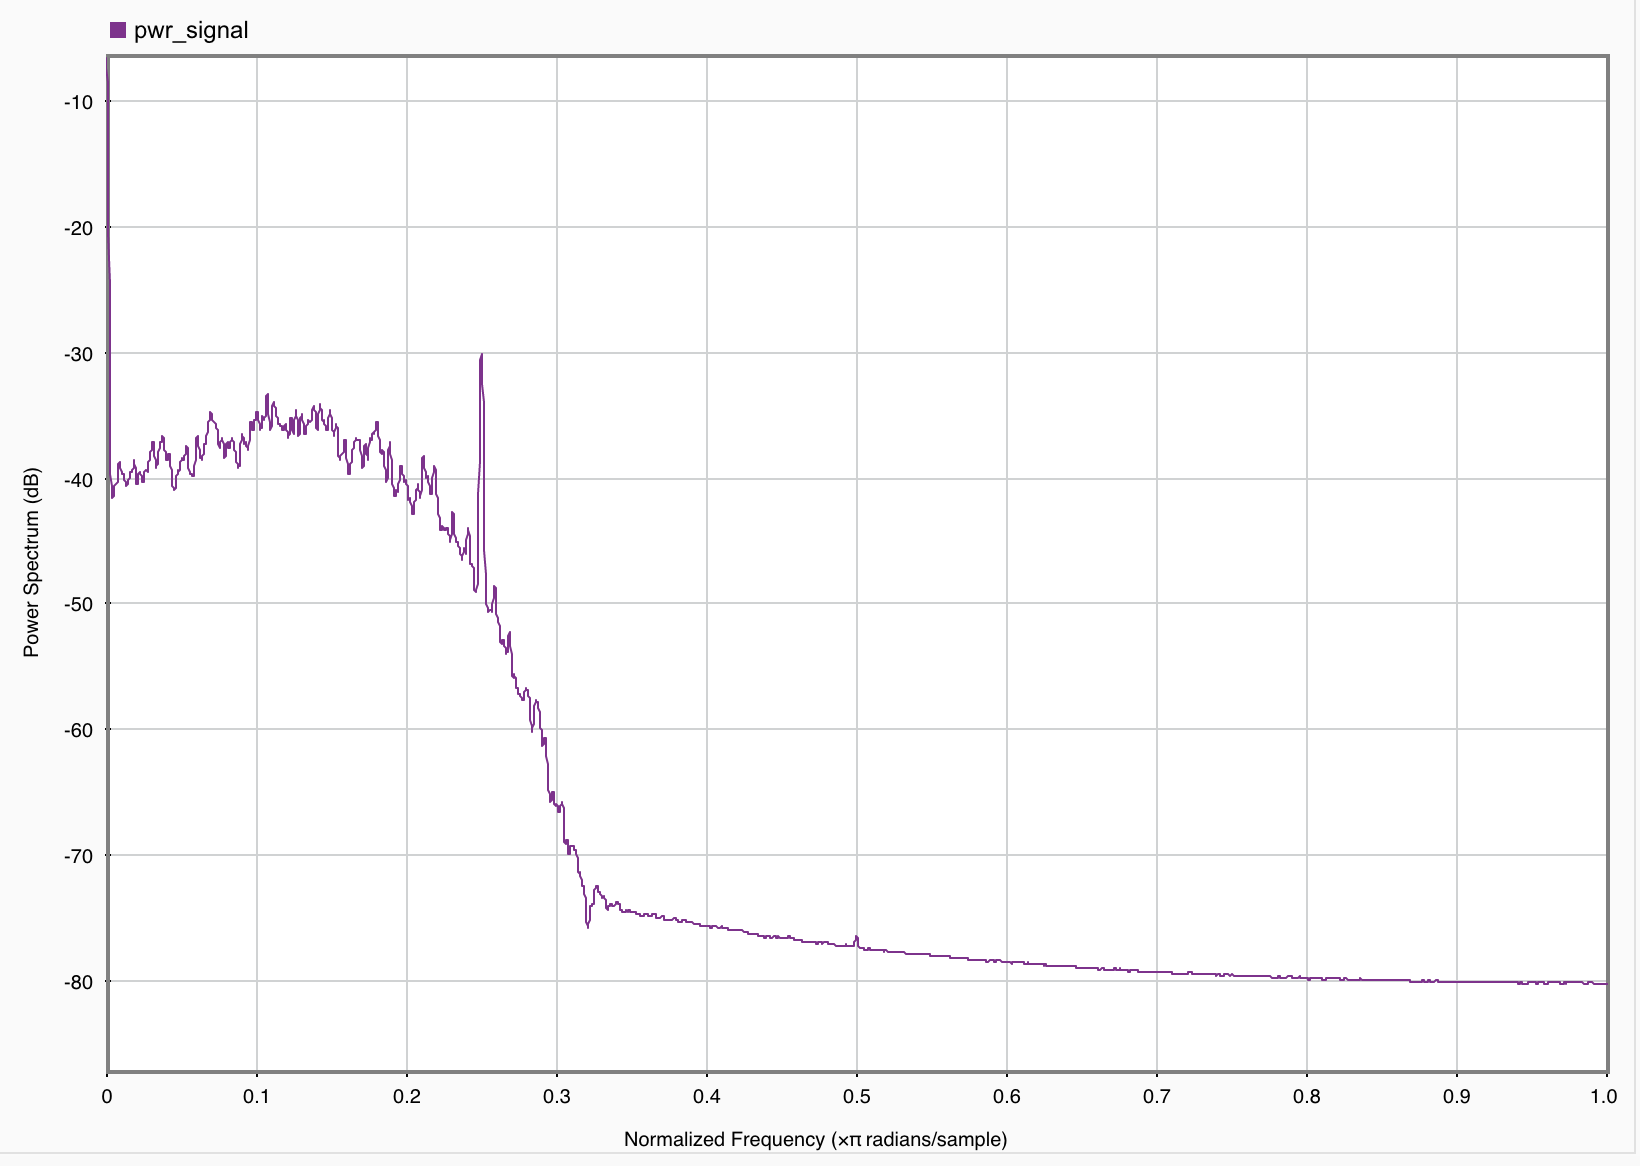
\includegraphics[width=\figW\linewidth]{spectrum.png}
\caption{Received signal power spectrum}
\label{fig:pwr_spectrum}
\end{center}
\end{figure}

The system delay was measured by transmitting a known bit sequence and evaluating the time delay from sound producer to sound consumer. The delay was measured by running both the transmitter and receiver software on the same computer. The average measured delay was $\measDelay \si{ms}$ with a sample standard deviation of $\measDelayStd \si{ms}$.  

\subsection{Performance Measurements}
\label{sec:perf_meas}
The system is testet in an indoor environment with both USRP's at the same altitude, 1 meter apart and no polarization mismatch. As the system us designed to change quality level depending on the state of the radio channel, different radio channels should be used when verifying the system performance. However, for the sake of reproducibility, we chose to vary the received SNR by adjusting the transmit power instead of changing the radio channel. Two different transmit power levels was used to verify transmission at both qualities. High quality transmission was measured with a transmit power of $\measPWR \si{dBm}$ and low quality with $\measPWRbad \si{dBm}$. 

Eye diagram and constellation diagram is provided for both transmit power levels and both modulation formats, together with some key performance measurements. For each transmit power level, the BER is calculated by transmission of a known bit sequence and the average EVM is calculated from constellation diagram, normalised to the average signal power. 

The diagrams for high and low transmit power are summarised in figure \ref{fig:good_diagrams} and \ref{fig:bad_diagrams} respectively. Calculated performance parameters are summarised in table \ref{tab:meas_params_good} and \ref{tab:meas_params_bad} for high and low transmit power respectively.

% !TEX root = main.tex
\begin{figure} 
    \centering
  \subfloat[QPSK constellation\label{1a}]{%
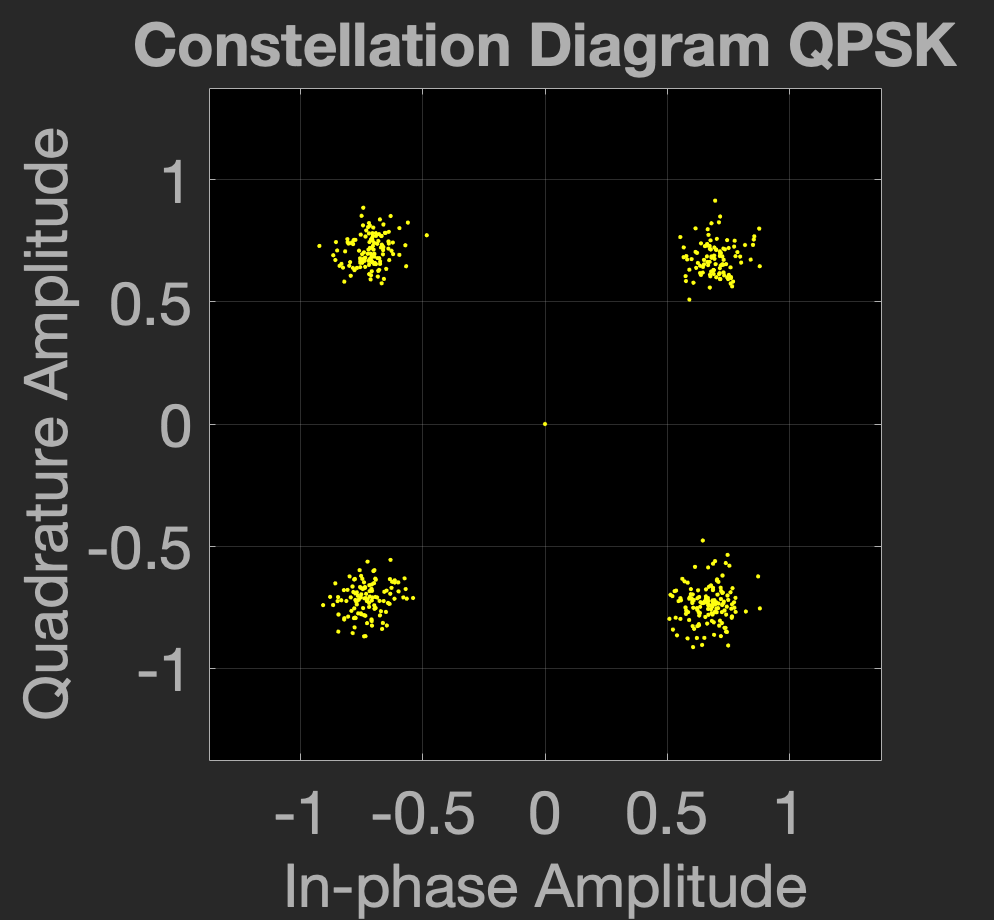
\includegraphics[width=0.45\linewidth]{constellationQPSKgood.png}
}
  \subfloat[QAM-16 constellation\label{1b}]{%
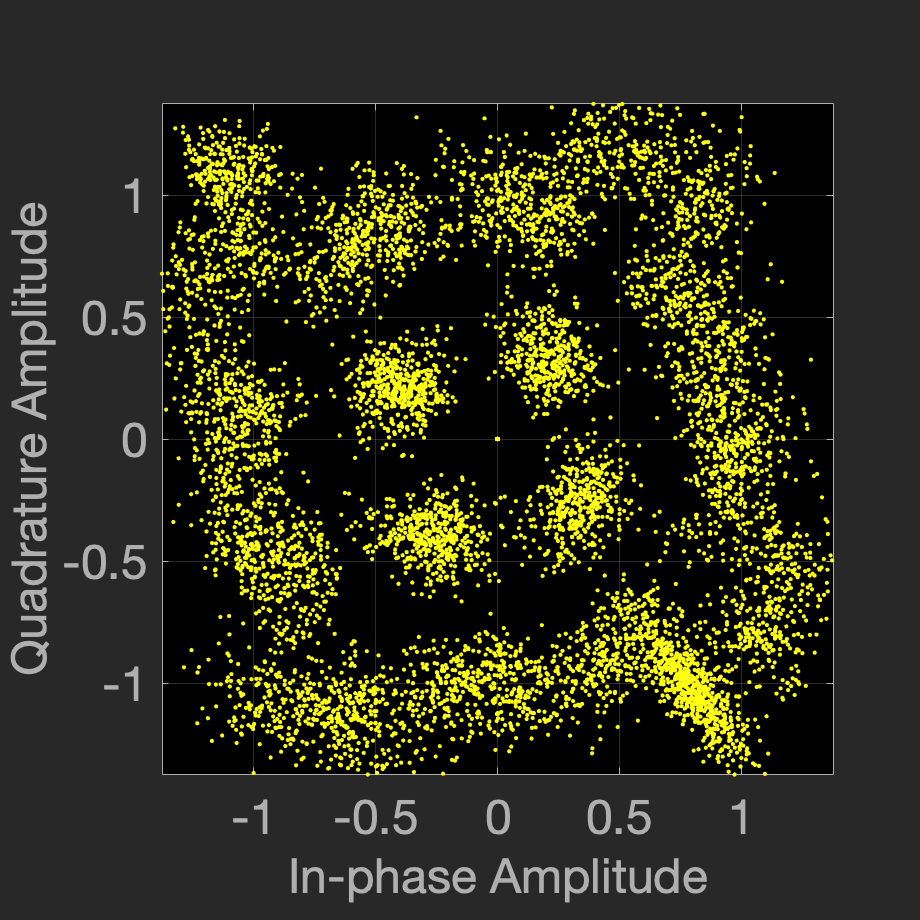
\includegraphics[width=0.45\linewidth]{constellationQAMgood.png}

}
\\
  \subfloat[QPSK eye diagram\label{1c}]{%
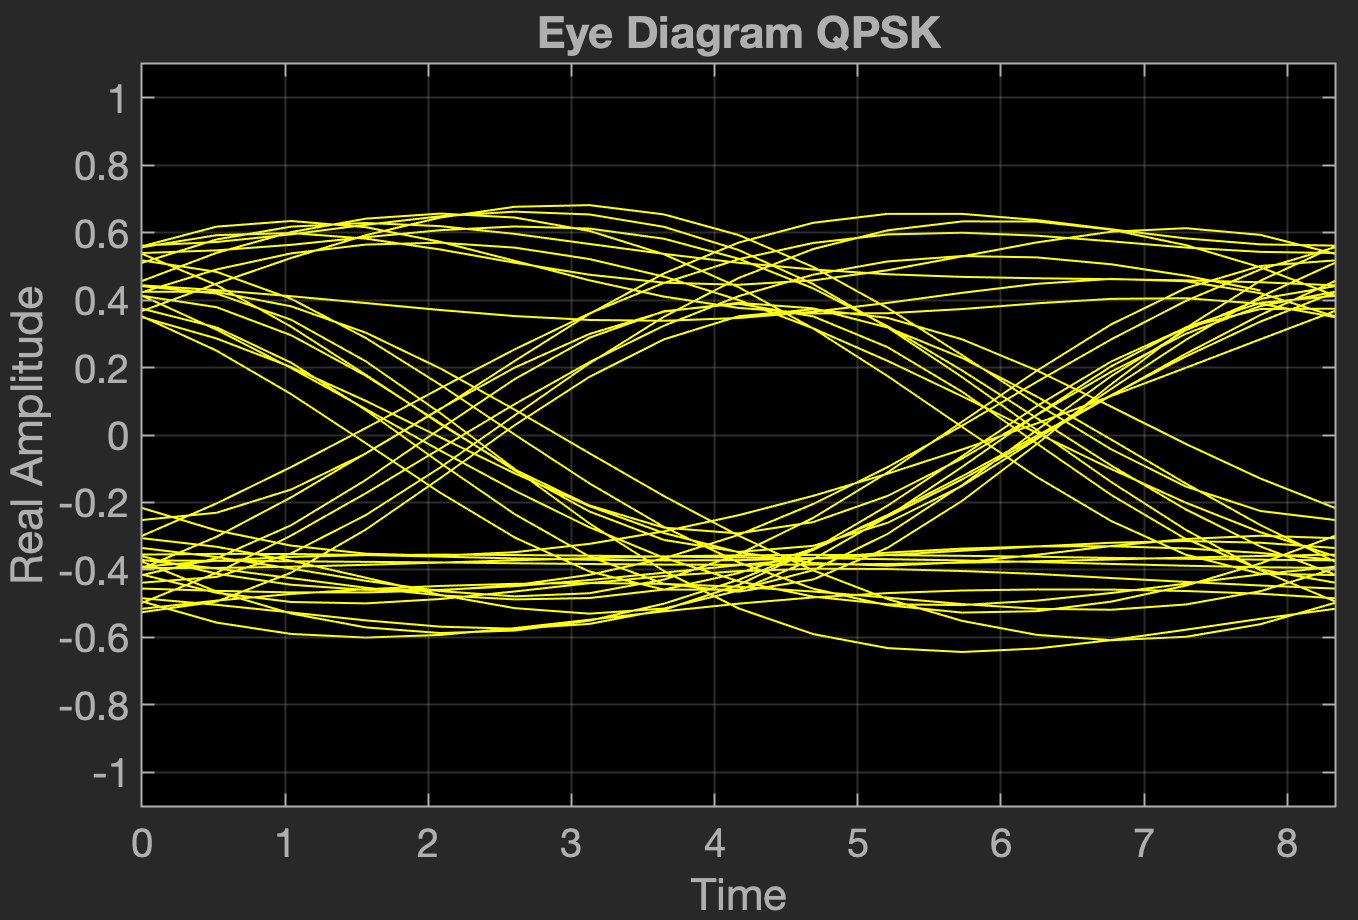
\includegraphics[width=0.45\linewidth]{eyeQPSKgood.png}

}
  \subfloat[QAM-16 eye diagram\label{1d}]{%
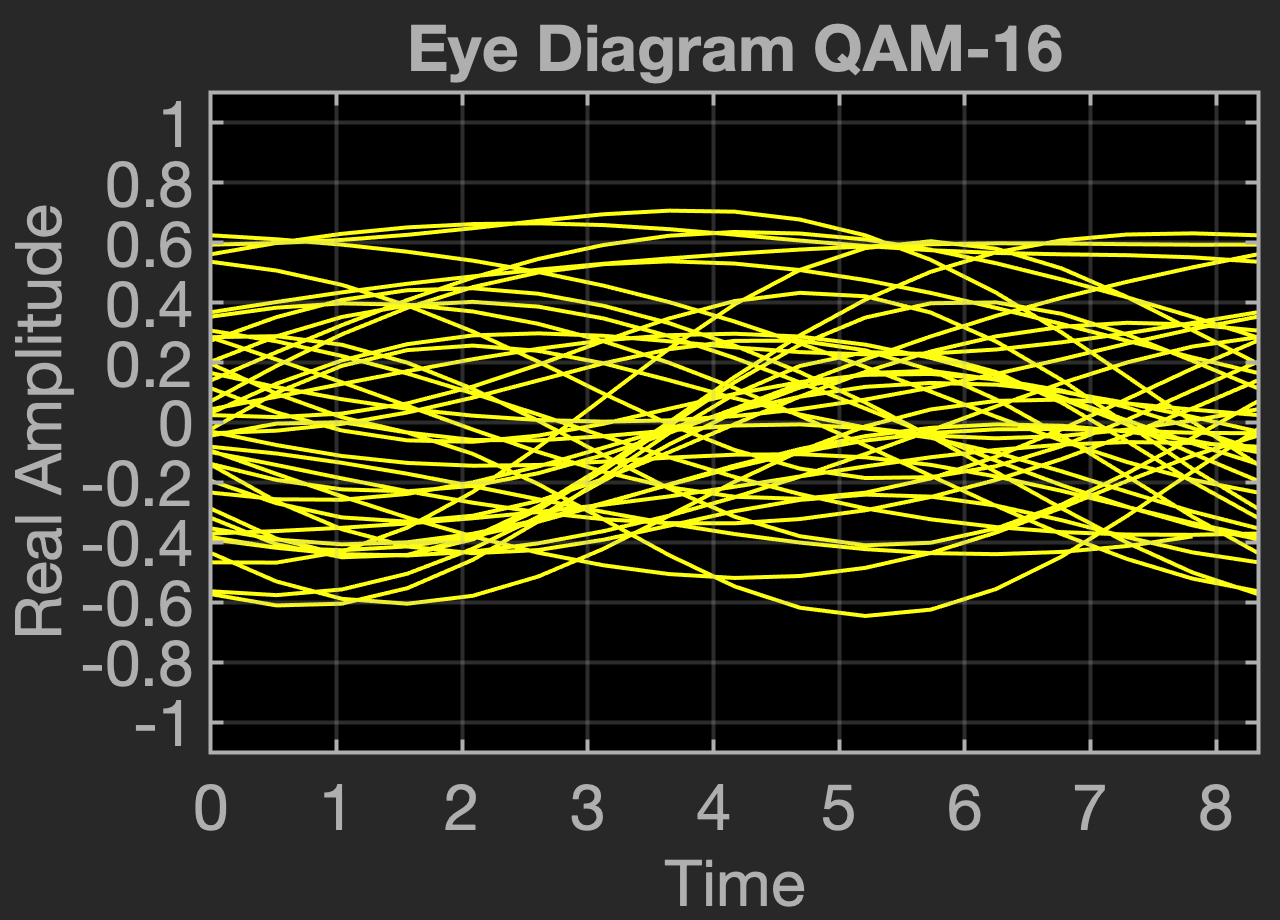
\includegraphics[width=0.45\linewidth]{eyeQAMgood.png}

}
  \caption{Eye diagram and constellation for QPSK (a and c) and QAM-16 (b and d) modulated symbols. Transmit power: \SI{\measPWR}{dBm}}
  \label{fig:good_diagrams} 
\end{figure}

% !TEX root = main.tex
\begin{figure} 
    \centering
  \subfloat[QPSK constellation\label{1a}]{%
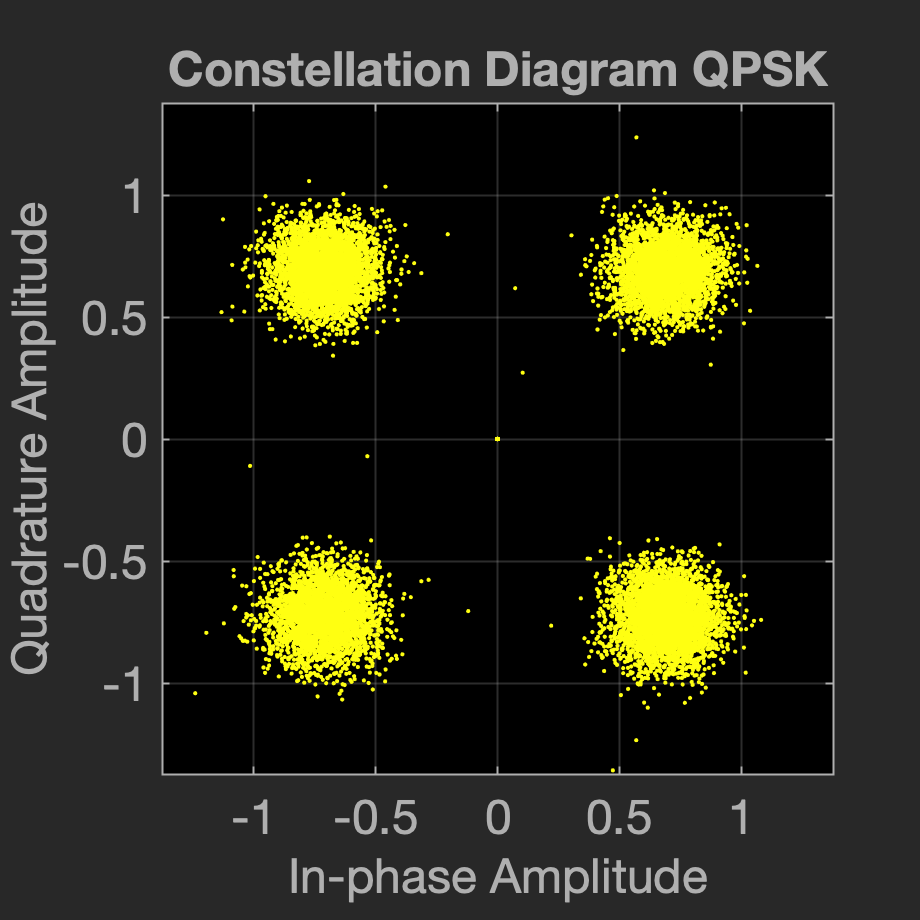
\includegraphics[width=0.45\linewidth]{constellationQPSKbad.png}
}
  \subfloat[QAM-16 constellation\label{1b}]{%
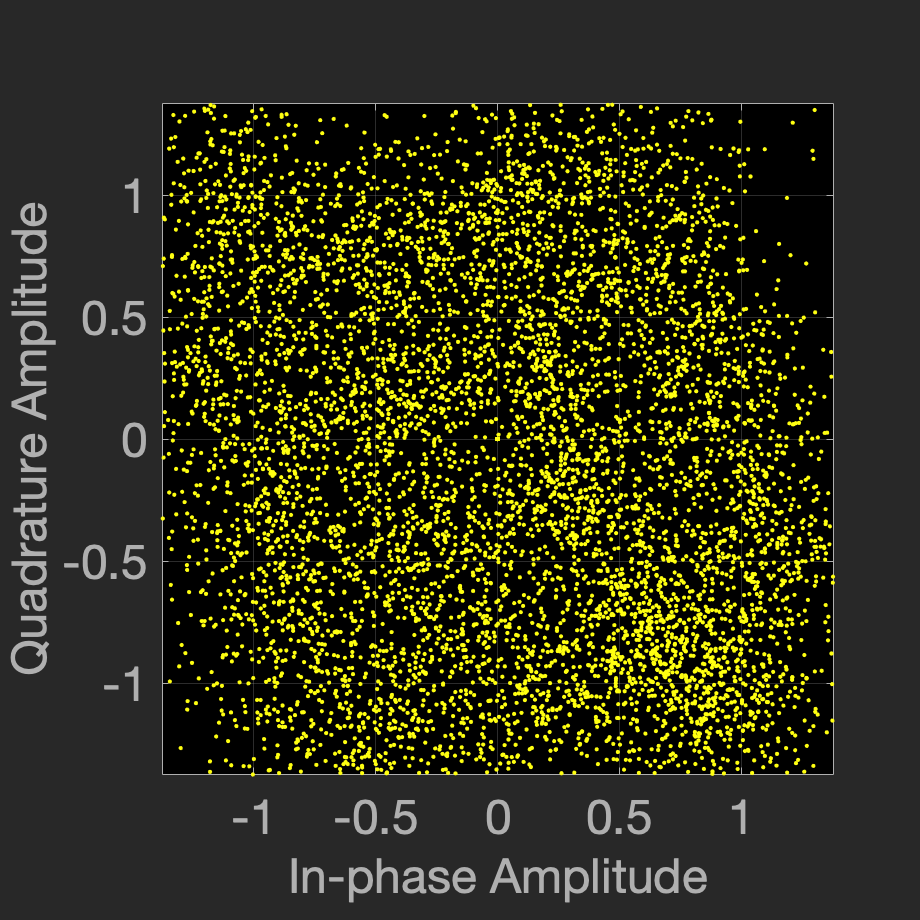
\includegraphics[width=0.45\linewidth]{constellationQAMbad.png}

}
\\
  \subfloat[QPSK eye diagram\label{1c}]{%
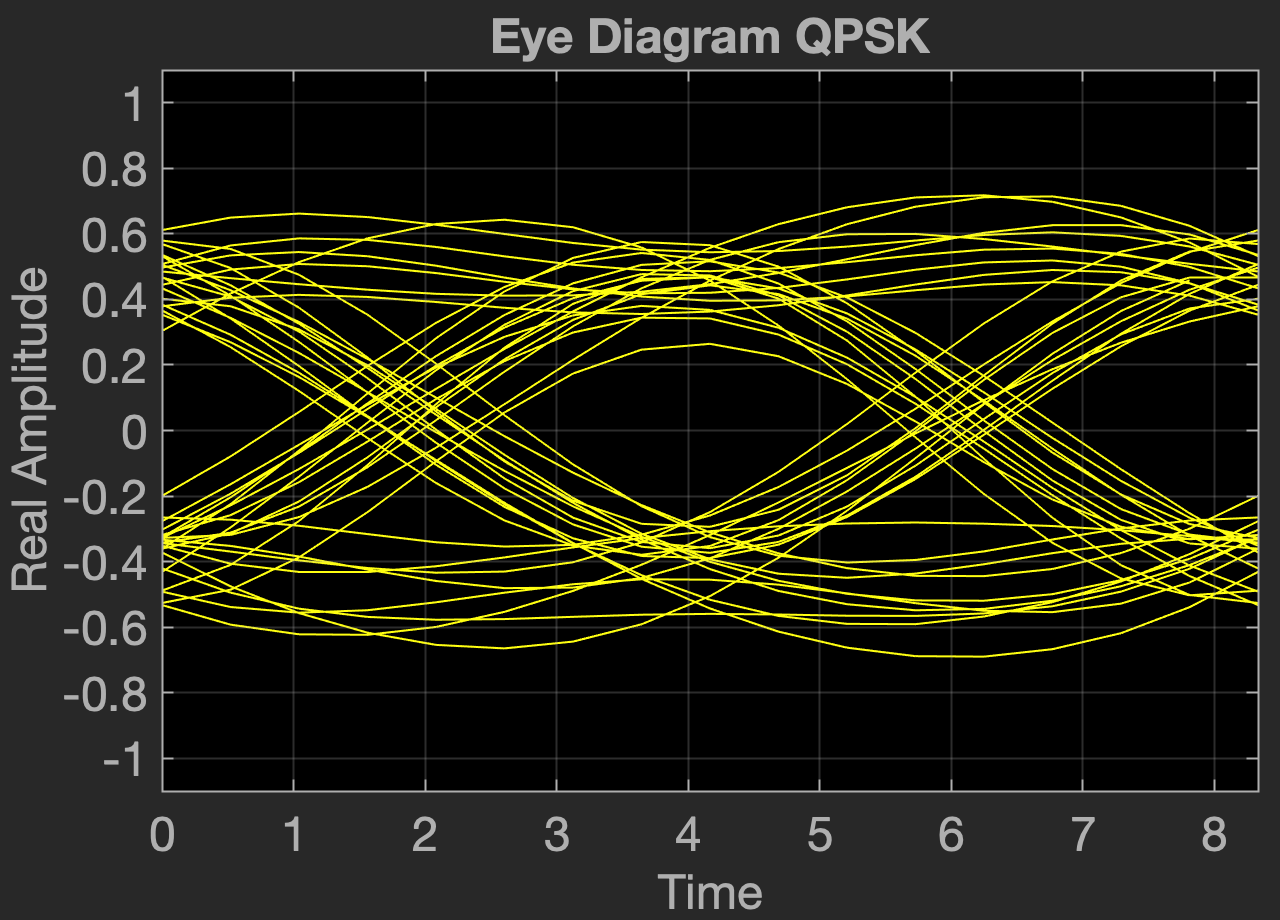
\includegraphics[width=0.45\linewidth]{eyeQPSKbad.png}

}
  \subfloat[QAM-16 eye diagram\label{1d}]{%
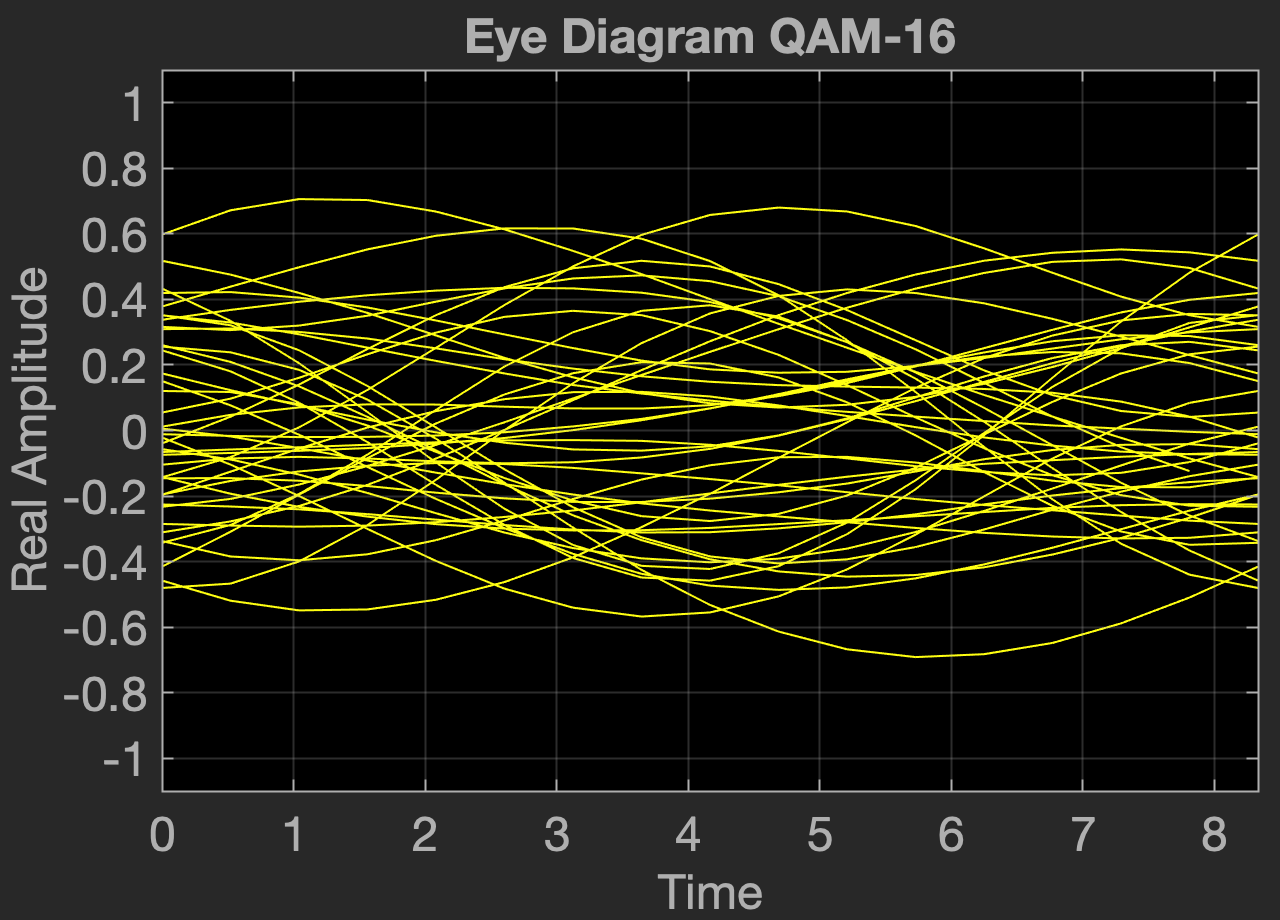
\includegraphics[width=0.45\linewidth]{eyeQAMbad.png}

}
  \caption{Eye diagram and constellation for QPSK (a and c) and QAM-16 (b and d) modulated symbols. Transmit power: $\measPWRbad \si{dBm}$}
  \label{fig:bad_diagrams} 
\end{figure}

% !TEX root = main.tex
\begin{table}[htbp]
  \centering
  \caption{Measured performance parameters. Transmit power: $\SI{\measPWR}{\decibel m}$}
    \begin{tabular}{lc}
    \rowcolor[rgb]{ 0,  0,  0} \textcolor[rgb]{ 1,  1,  1}{\textbf{System Parameter}}	& \textcolor[rgb]{ 1,  1,  1}{\textbf{Measured Value}} 		\\
    \rowcolor[rgb]{ 0,  0,  0} \textcolor[rgb]{ 1,  1,  1}{} & \textcolor[rgb]{ 1,  1,  1}{\textbf{Modulation QPSK / QAM-16}}					\\
    	SNR 													& $\SI{\measSNRQPSKGood}{dB} / \SI{\measSNRQAMGood}{dB}$							\\
	\ebnot 													& $\SI{13.1}{dB} /\SI{4.6}{dB}$							\\
    	BER			 											& \measBERQPSKGood / \measBERQAMGood 		\\
	EVM 													& $\SI{-17.5}{dB} / \SI{-14.5}{dB}$							\\

 \end{tabular}
  \label{tab:meas_params_good}
\end{table}
% !TEX root = main.tex
\begin{table}[htbp]
  \centering
  \caption{Measured performance parameters. Transmit power: $\measPWRbad \si{dBm}$}
    \begin{tabular}{lc}
    \rowcolor[rgb]{ 0,  0,  0} \textcolor[rgb]{ 1,  1,  1}{\textbf{System Parameter}}	& \textcolor[rgb]{ 1,  1,  1}{\textbf{Measured Value}} 		\\
    \rowcolor[rgb]{ 0,  0,  0} \textcolor[rgb]{ 1,  1,  1}{} & \textcolor[rgb]{ 1,  1,  1}{\textbf{Modulation QPSK / QAM-16}}					\\

    	SNR														& $\measSNRGood\si{dB}$						\\
    	EVM 													& $\measEVMGood \si{dB}$						\\
    	BER			 											& \measBERQPSKGood / \measBERQAMGood		\\
 \end{tabular}
  \label{tab:meas_params_bad}
\end{table}

\subsection{Quality of Service}
We conclude this section with a qualitative description of the perceived quality of service (QoS). This is the best radio system ever made. People are surprised how good this system is. Nobody knows radio systems better than us.   

